    %----------------------------------------------------------------------------------------
    %    PACKAGES AND THEMES
    %----------------------------------------------------------------------------------------

    \documentclass{beamer}
    \usepackage{graphicx}
    \usepackage{ragged2e}
    \usetheme{Madrid}
    \usepackage{caption}
    \setbeamercolor{background canvas}{bg=white}
    \setbeamercolor{normal text}{fg=black}
    \setbeamertemplate{footline}[frame number]
    \addtobeamertemplate{footline}{\ifnum\value{framenumber}=1\else\hspace*{\fill}\fi}{}
    \definecolor{LightCyan}{rgb}{0.87, 0.87, 0.87}
    \setbeamercolor{section in toc}{fg=black}
    \setbeamercolor{subsection in toc}{fg=black}
    \setbeamertemplate{caption}[numbered]
    \setbeamercolor{headline}{bg=white}
    \setbeamercolor{title}{fg=black}
    \setbeamercolor{frametitle}{bg=white, fg=black}
    \usepackage{svg}
    \usepackage[T2A]{fontenc}
    \usepackage[utf8]{inputenc}
    \usepackage[english,russian]{babel}
    \usepackage{longtable}
    % \title{Визуализация процесса извержения вулкана}
    % \author{Бугаков Иван Сергеевич}
    % \institute{МГТУ им. Н. Э. Баумана}
    % \date{2025 г.}
    \setbeamertemplate{navigation symbols}{}
    \usepackage{ragged2e}
    \let\raggedright=\RaggedRight
    \usepackage{colortbl}
    \usepackage{xcolor}
    \usepackage{tikz}
    \hyphenation{тех-но-ло-гия}
    \begin{document}
    \setbeamertemplate{frametitle}[default][center]

    %----------------------------------------------------------------------------------------
    %    TITLE PAGE
    %----------------------------------------------------------------------------------------

    \begin{frame}[noframenumbering,plain]
        \begin{columns}[t!] % создаем две колонки
            % Первая колонка для логотипа
            \begin{column}{0.2\textwidth}
                
\includegraphics[width=2.5cm]{assets/logo.png} % Укажите путь к логотипу
            \end{column}
            % Вторая колонка для текста
            \begin{column}{0.8\textwidth}
            \centering
                {\footnotesize Министерство науки и высшего образования Российской Федерации\\
                
                Федеральное государственное бюджетное образовательное учреждение высшего образования\\
                
                «Московский государственный технический университет
                имени Н.~Э.~Баумана
                (национальный исследовательский университет)» \\
                
                (МГТУ им.~Н.~Э.~Баумана)} 
            \end{column}
        \end{columns}
        \vfill
        \centering
        {\LARGE \textbf{Разработка базы данных для хранения и обработки оценок трудовой эффективности сотрудников группы компаний}} \\
        \vfill

        \raggedleft
        {\large Группа: ИУ7-64Б} \\
        
        {\large Студент: Бугаков Иван Сергеевич} \\
        
        {\large Научный руководитель: Гончаров Сергей Сергеевич} \\
        \vfill
        \centering
        {\small 2025 г.}

    \end{frame}

    \setcounter{framenumber}{1}
    \begin{frame}{\centeringЦель и задачи работы}
        \textbf{Цель работы}~---~разработка базы данных для хранения и обработки оценок трудовой эффективности сотрудников группы компаний.\\
        \vfill
        \textbf{Задачи:}
        \begin{itemize}
        \item[---] провести анализ предметной области, выделить основные сущности и связи между ними, сформулировать требования и ограничения к разрабатываемой базе данных;
        \item[---] спроектировать сущности базы данных и определить ограничения целостности данных, спроектировать ролевую модель на уровне базы данных;
        \item[---] выбрать средства реализации базы данных и приложения;
        \item[---] реализовать сущности базы данных и ограничения целостности. Описать методы тестирования и разработать тестовые случаи для проверки корректности работы функционала;
        \item[---] провести исследование производительности базы данных при увеличении объема данных и количестве одновременно выполняемых запросов, а также с использованием кеширования и без него.    
    \end{itemize}
    \end{frame}
    \begin{frame}{\LARGE Требования к базе данных}
    База данных должна предоставлять возможность хранения и обработки:
    \begin{itemize}
    \item[---] оценок работников группы компаний по критериям непосредственно эффективности, вовлеченности и компетенции;
    \item[---] информации о сотрудниках;
    \item[---] информации о компаниях группы;
    \item[---] должностях и позициях занимаемых сотрудниками и историях их изменения.
    \end{itemize}
    \end{frame}
    \begin{frame}{Выбор трехмерной модели}
    \begin{figure}
        \centering
        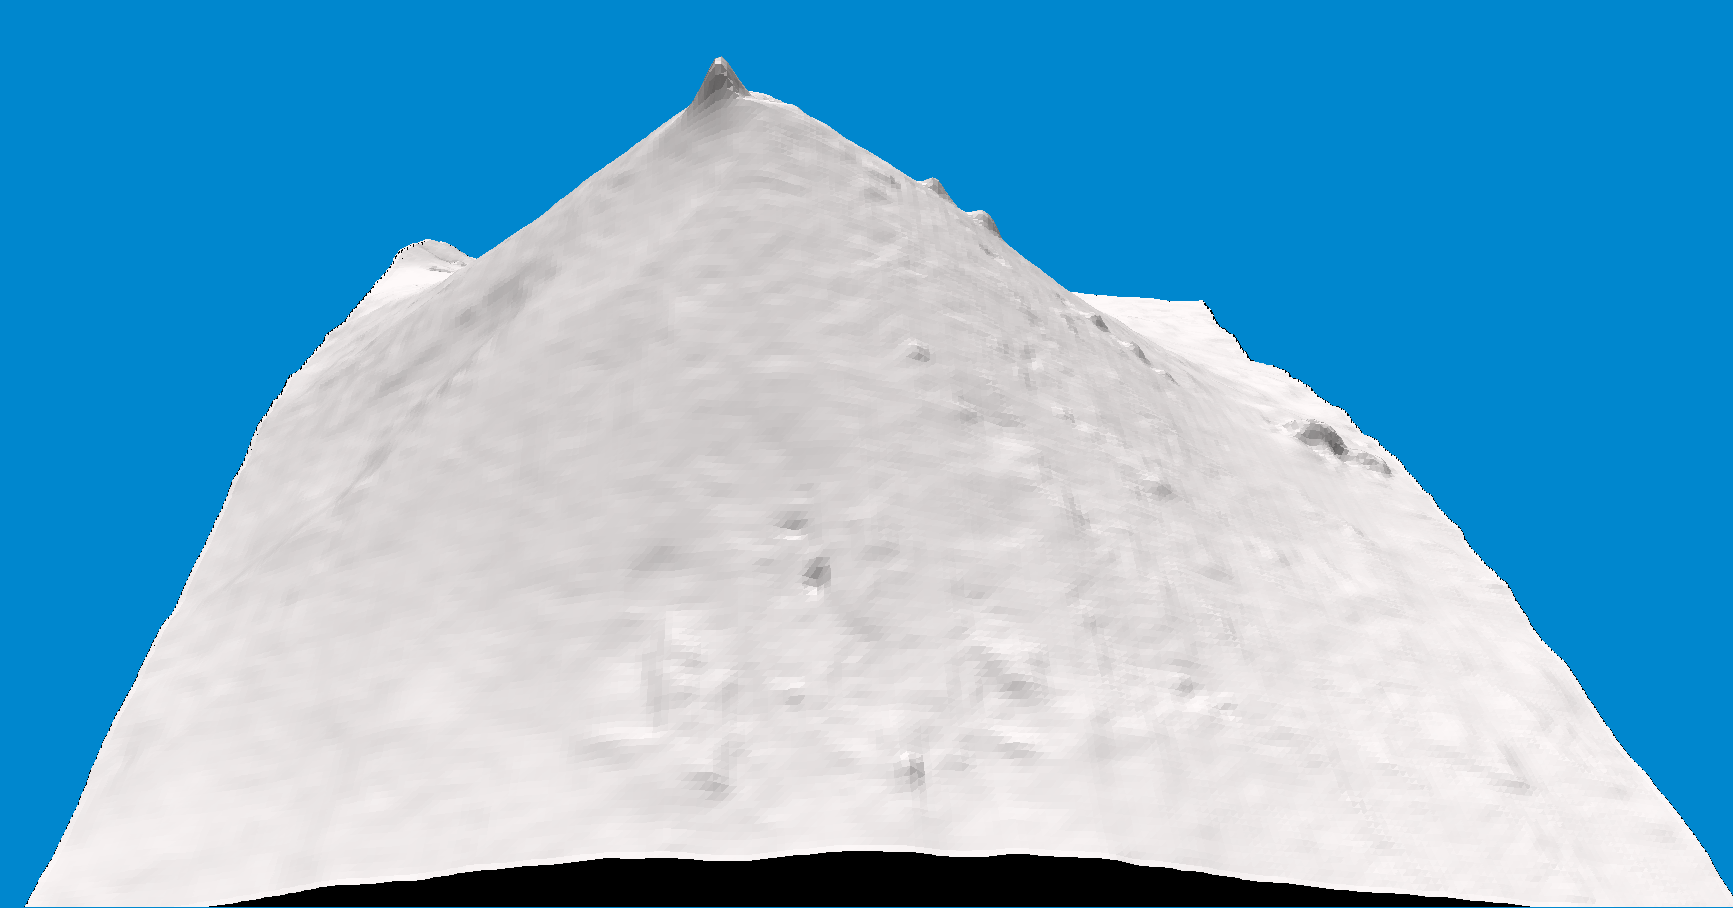
\includegraphics[width=0.5\linewidth]{assets/model.png}
    \end{figure}

    Для визуализации вулкана была выбрана поверхностная модель, в связи с распространенностю STL-моделей для представления карты высот реального ландшафта земной поверхности, полученной в результате радарной спутниковой топографической съемки. 
    \end{frame}
    \begin{frame}{Выбор модели движения дыма}
        \begin{longtable}{|l|c|c|}
        \hline
        \textbf{Модель} & \textbf{Скорость} & \textbf{Ресурсоемкость} \\
        \hline
        Система чистиц & Низкая & Высокая\\
        \hline
        \rowcolor{LightCyan}
        Уравнения Навье---Стокса & Средняя & Средняя \\
        \hline
    \end{longtable}

    В результате анализа была выбрана модель на основе уравнений Навье---Стокса.
    \end{frame}
    \begin{frame}{Модель движения дыма}
        Уравнения Навье --- Стокса — система дифференциальных уравнений в частных производных, описывающая движение вязкой ньютоновской жидкости.
        \begin{columns}[t]
            \begin{column}{0.5\textwidth}
                \textbf{\textit{Уравнение скорости}} определяет изменение поля скорости во времени:
                $$
                    \frac{\partial \vec{u}}{\partial t} = - (\vec{u} \cdot \nabla) \vec{u} + \nu \nabla^2 \vec{u} + f.$$ 
                \begin{itemize}
                {\small
        \item [---] $\frac{\partial \vec{u}}{\partial t}$ --- производная скорости по времени;
        \item[---] $(\vec{u} \cdot \nabla) \vec{u}$ --- изменение скорости из-за движения дыма;
        \item[---] \(\nu \nabla^2 \vec{u}\) --- вязкость (диффузия);
        \item[---] \(\vec{f}\) -- внешние силы.
        }
    \end{itemize}
            \end{column}
            \begin{column}{0.5\textwidth}
                \textbf{\textit{Уравнение плотности}} определяет изменение распределения плотности во времени:
        $$\frac{\partial \rho}{\partial t} = -(\vec{u} \cdot \nabla) \rho + \kappa \nabla^2 \rho + S.$$ 
    \begin{itemize}
    {\small
        \item[---] \(\rho\) --- плотность жидкости или газ;
        \item[---] \((\vec{u} \cdot \nabla) \rho\) --- изменение плотности дыма из-за потока жидкости или газа;
        \item[---] \(\kappa \nabla^2 \rho\) --- диффузия дыма;
        \item[---] \(S\) --- источник дыма.
        }
    \end{itemize}
            \end{column}
        \end{columns} 
    \end{frame}
    \begin{frame}{Модель освещения}
        Для визуализации освещения была выбрана модель на основе закона Ламберта:
        $$
        I = I_l k_d \cos(\theta).
        $$
        \begin{itemize}
        \item[---] $I$ — интенсивность отраженного света,  
        \item[---] $I_l$ — интенсивность падающего света от точечного источника,  
        \item[---] $k_d$ — коэффициент диффузного отражения,  
        \item[---] $\theta$ — угол между направлением падающего света $L$ и нормалью к поверхности $N$.  
    \end{itemize}

    Эта модель была выбрана, так как STL-модели не предоставляют никаких сведений о материале объекта визуализации.
    \end{frame}
    \begin{frame}{Алгоритмы визуализации}

    \centering
        \begin{tabular}{|l|l|}
            \hline
            \textbf{Задача} & \textbf{Алгоритм решения}\\
            \hline
            {\small
            Удаление невидимых линий и поверхностей & Z-буфер \\
            \hline
            Модель освещения & Ламберта \\
            \hline
            Модель поведения дыма & Уравнения Навье---Стокса \\
            \hline
            }
        \end{tabular}
        
    \end{frame}
    \begin{frame}{Схема алгоритма, использующего z-буфер}
    \begin{figure}
        \centering
        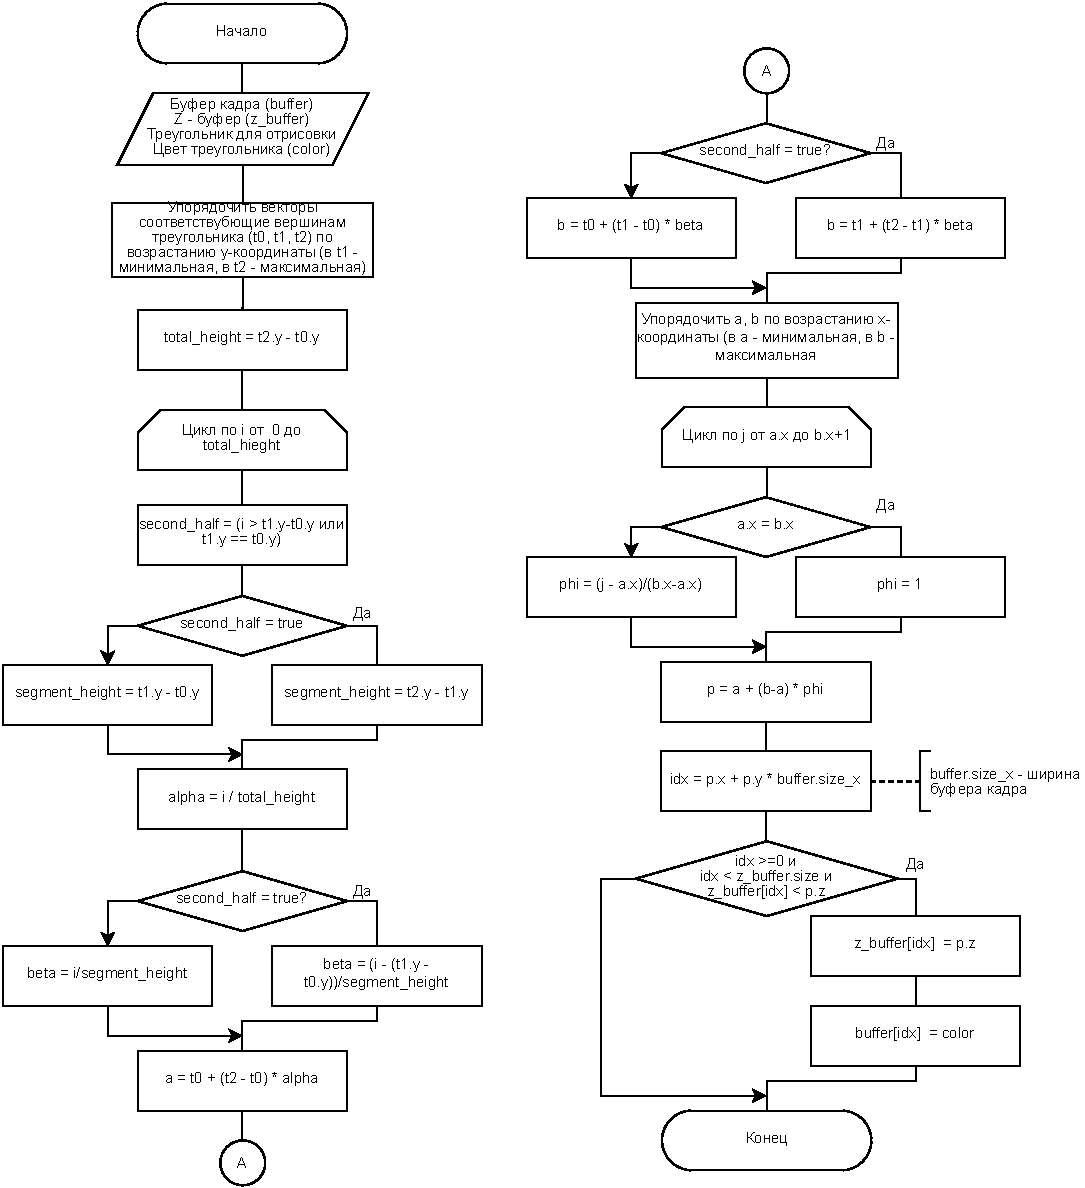
\includegraphics[width=0.6\linewidth]{assets/z-bufer-full.pdf}
    \end{figure}
    \end{frame}
    \begin{frame}{Схема алгоритма на основе уравнений Навье---Стокса}
        \begin{figure}[htb!]
            \centering
            \begin{minipage}{0.3\textwidth}
                \centering
                    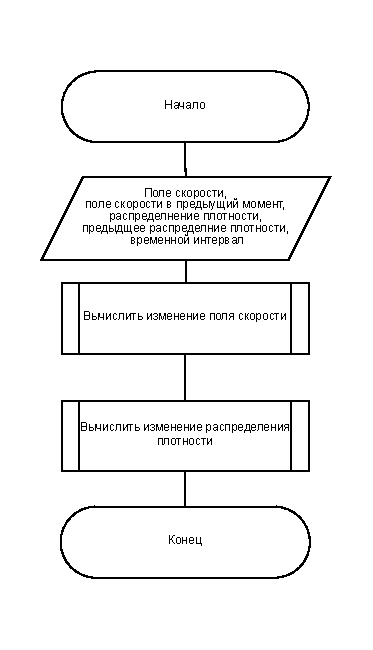
\includegraphics[height=1.0\textheight, width=\textwidth, keepaspectratio]{assets/Naive_stocks.pdf}
                    
                % \caption*{Общий вид алгоритма}
                    \centering
            \end{minipage}
            \begin{minipage}{0.3\textwidth}
                    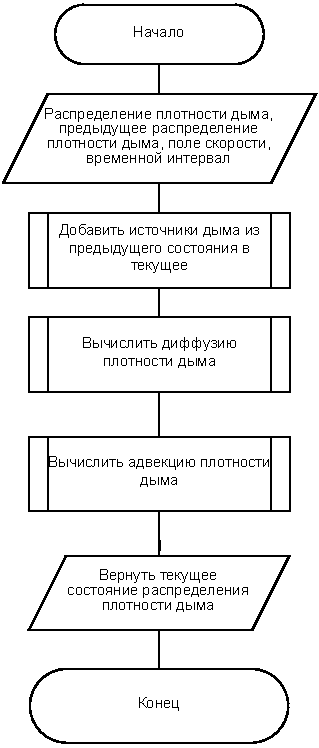
\includegraphics[height=0.7\textheight, width=\textwidth, keepaspectratio]{assets/dens_step.pdf}
            % \caption*{Вычиление изменения распределения плотности}
                \end{minipage}
                \begin{minipage}{0.3\textwidth}
                    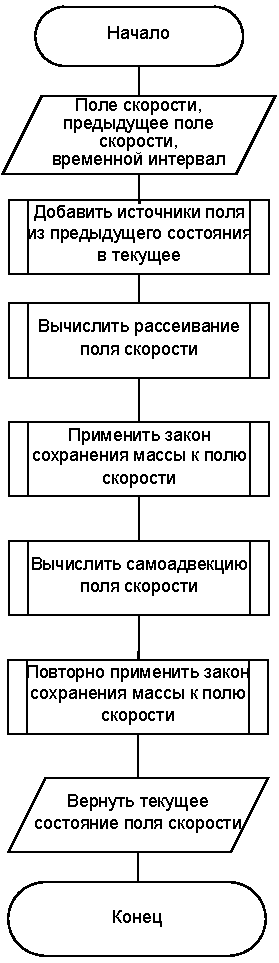
\includegraphics[height=0.7\textheight, width=\textwidth, keepaspectratio]{assets/velocity_step.pdf}
                    
                % \caption*{Вычисление изменения поля скорости}
                \end{minipage}
        \end{figure}
        \begin{columns}[t]
            \begin{column}{0.3\textwidth}
                Общий вид алгоритма
            \end{column}
            \begin{column}{0.3\textwidth}
            Вычиление изменения распределения плотности
                \end{column}
                \begin{column}{0.3\textwidth}
                    Вычисление изменения поля скорости
                \end{column}
        \end{columns} 
    \end{frame}
    \begin{frame}{Диаграмма классов}
        \begin{figure}
        \centering
        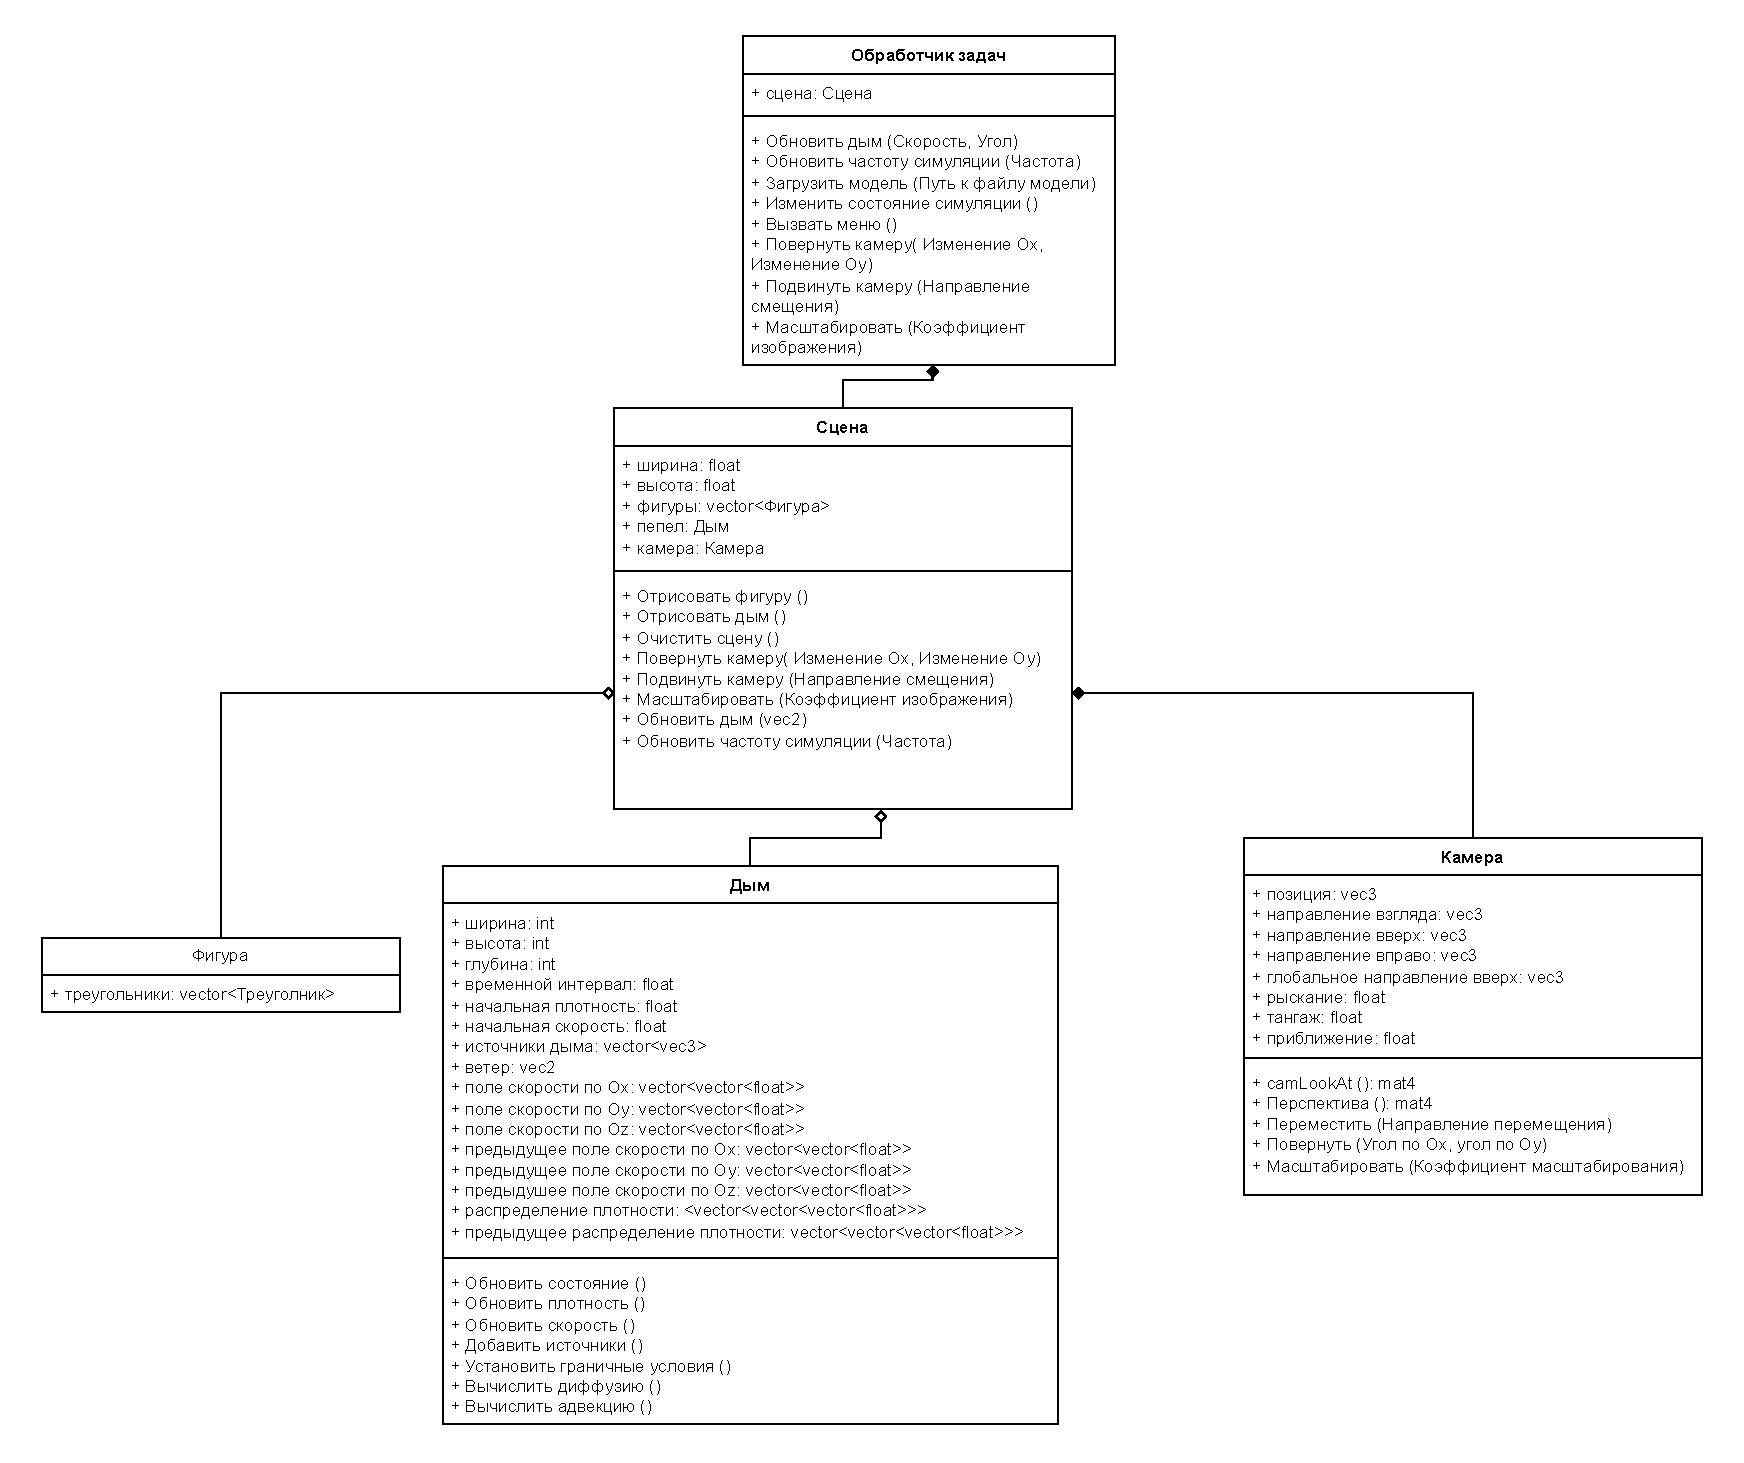
\includegraphics[width=0.8\linewidth]{assets/smoke_uml.pdf}
    \end{figure}
    \end{frame}
    \begin{frame}{Реализация алгоритмов}
        Язык программирования --- С++.
        
        Графический интерфейс --- Qt.
        
        Визуализация --- SFML.
        
        Параллельные вычисления --- OpenMP.
    \end{frame}
    \begin{frame}{Результат работы программы}
            \begin{figure}
        \centering
        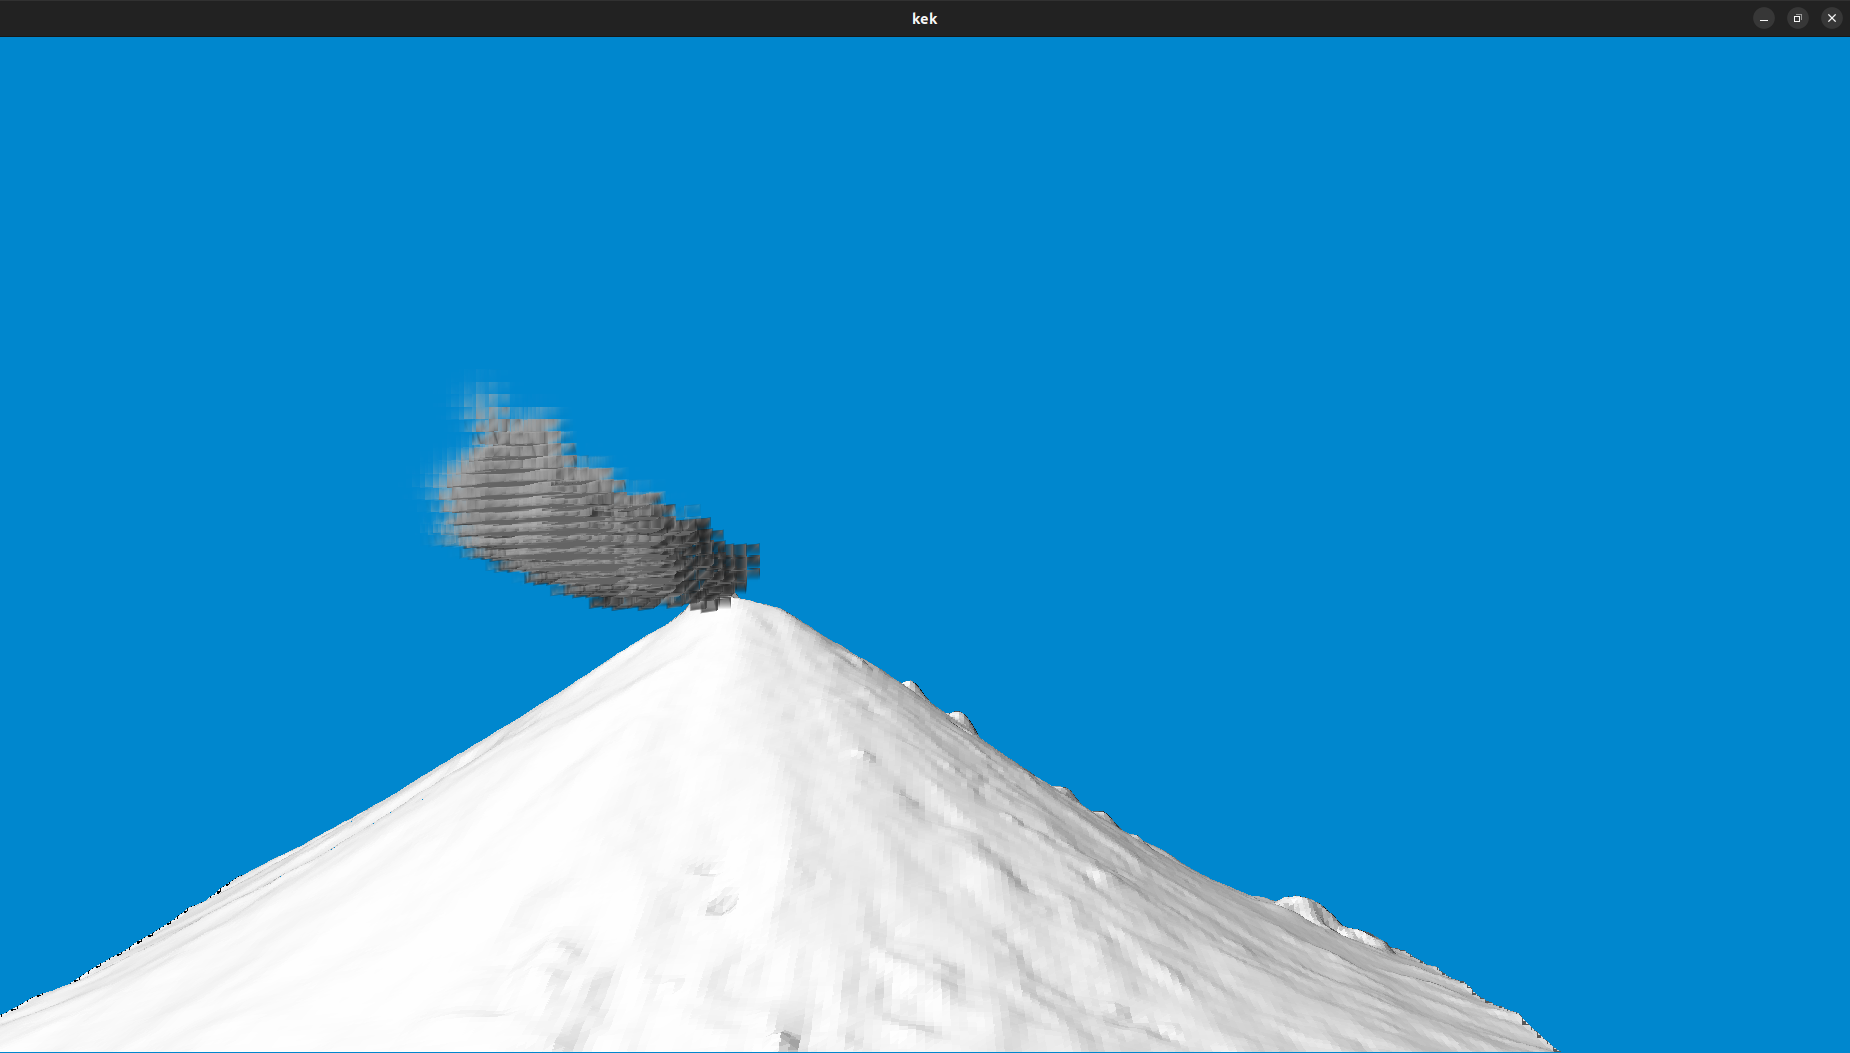
\includegraphics[width=1.0\linewidth]{assets/visualization.png}
    \end{figure}
    \end{frame}
    \begin{frame}{Исследование}
        \begin{minipage}{0.48\textwidth}
        \begin{figure}
            \centering
            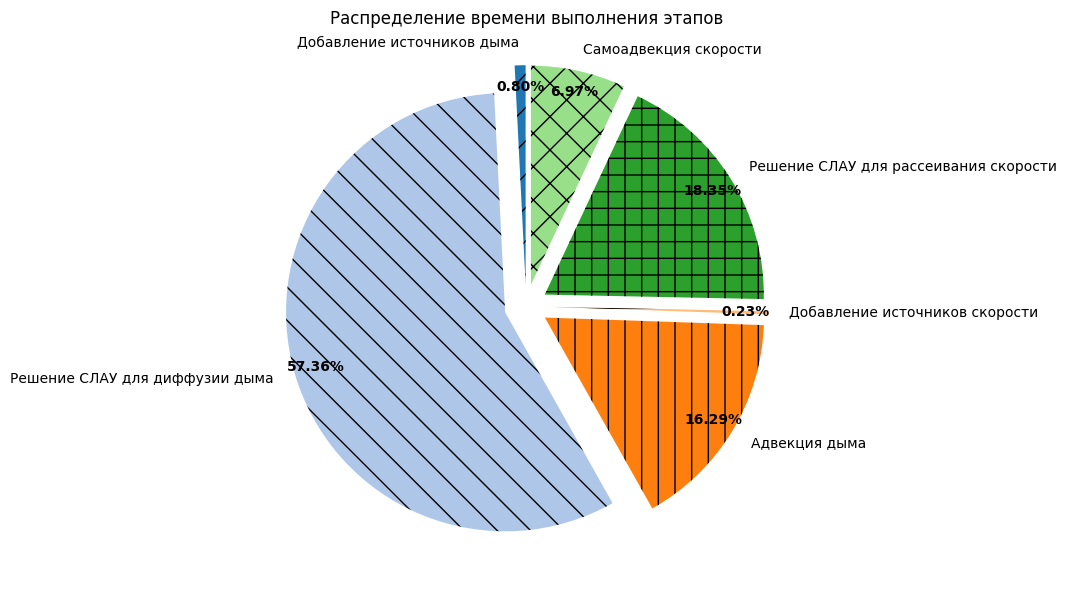
\includegraphics[width=1.0\linewidth]{assets/pie.png}
            \caption*{Без параллельных вычислений общее время работы --- 0.372 сек}
        \end{figure}
    \end{minipage}
    \begin{minipage}{0.48\textwidth}
            \begin{figure}
            \centering
            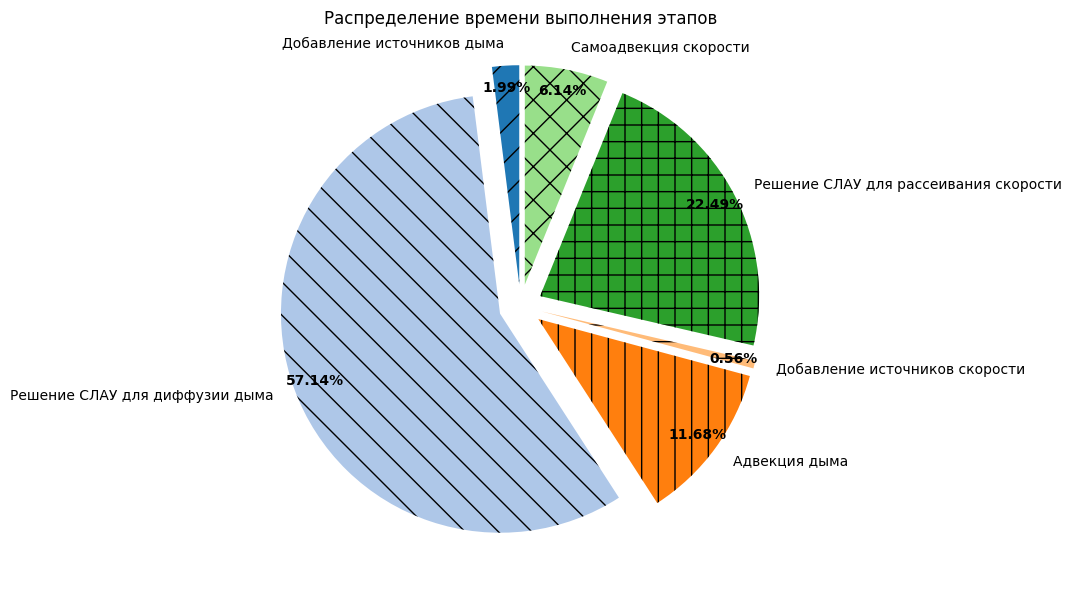
\includegraphics[width=1.0\linewidth]{assets/pie_parallel.png}
            \caption*{С параллельными вычислениями общее время работы --- 0.185 сек}
        \end{figure}
    \end{minipage}

    Наиболее длительными частями алгоритма являются решения СЛАУ и вычисления адвекций. Применение к ним параллельных вычислений позволяет добиться двухкратного ускорения работы алгоритма.
    \end{frame}
    \begin{frame}{Заключение}
        Цель курсовой работы -- разработка программного обеспечения для визуализации процесса извержения вулкана --- была достигнута.
        Для этого были выполнены поставленные задачи:
        \begin{itemize}
        \item[---] проведен анализ алгоритмов  удаления невидимых линий и поверхностей, построения освещения, визуализации и выбраны наиболее подходящие для решения задачи;
        \item[---] спроектировано программное обеспечение;
        \item[---] выбраны средства реализации программного обеспечения и проведена его разработка;
        \item[---] проведено исследование характеристик разработанного программного обеспечения.
    \end{itemize}
    \end{frame}
    \end{document}